\documentclass{standalone}
\usepackage{tikz}
\usepackage{pgfplots}
\pgfplotsset{compat=newest}
\usetikzlibrary{calc}
\usepackage{ifthen}
\newcommand\mycolor{white}
\usetikzlibrary{matrix}

\newcommand\txbox[2]{
    \def\x{3}
    \def\y{2.5}
    \def\h{0.5}
    \def\A{{#1}}
    \node[anchor=north west] (B) at (\A) {$payload$};
    \node[anchor=north west] (C) at ($(\A) + (0,-\h)$) {$script$};
    \node (T) at ($(\A) + (8.75*\h,0.5*\h)$) {Output[0]};
    \node (I) at ($(\A) + (-2.3*\h,-0.6*\h)$) {Input[x{#2}]};
    \foreach \i in {1,...,14}
    {
        \draw ($(\A) + ({(\i+2)*\h},0)$) 
                    rectangle 
                    ($(\A) + ({(\i+3)*\h},-\h)$);
    }
    %\node[anchor=south west] (D) at ($(\A) + (1.9*\h,-2.1*\h)$) {$(R2==self.R2)
    %\wedge( R1== Rule110(self.R1) )$};
    \draw ($(\A) + (0,-\h)$) -- ($(\A) + (\x,{-\h})$);
    \draw ($(\A) + (3*\h,0)$) -- ($(\A) + (3*\h,-2*\h)$);
    \draw ($(\A)$) rectangle ($(\A) + (17*\h,-2*\h)$);
    \draw[fill=gray!50] ($(\A) + (3*\h,-\h)$) rectangle ($(\A) + (17*\h,-2*\h)$);
    \draw ($(\A) + (-0.2*\h, \h)$) rectangle ($(\A) + (17.2*\h,-2.2*\h)$);
    \draw[very thick] ($(\A) + (-4*\h, 2.5*\h)$) rectangle ($(\A) + (17.4*\h,-4*\h)$);
    \draw ($(\A) + (-3.8*\h, \h)$) rectangle ($(\A) + (-0.8*\h,-2.2*\h)$);
    \draw ($(\A) + (-4*\h, 1.5*\h)$) -- node[above, midway] {Transaction {#2}} ($(\A) + (17.4*\h,1.5*\h)$);
    \draw[densely dotted, very thick] ($(\A) + (-0.8*\h, -0.6*\h)$) -- ($(\A) + (-0.2*\h,-0.6*\h)$);
    \node (NN) at ($(\A) + (6.7*\h,-3*\h)$) {$\cdots$};
}

\newcommand\chainArr[4]{
    \draw[very thick, >=stealth,->] ({#1},{#2}) -- ({#1+0.5},{#2}) --
    ({#1+0.5},{0.5*#4+0.5*#2}) -- ({#3-0.5},{0.5*#4+0.5*#2}) -- 
    ({#3-0.5},{#4}) -- ({#3},{#4});
}

\begin{document}
    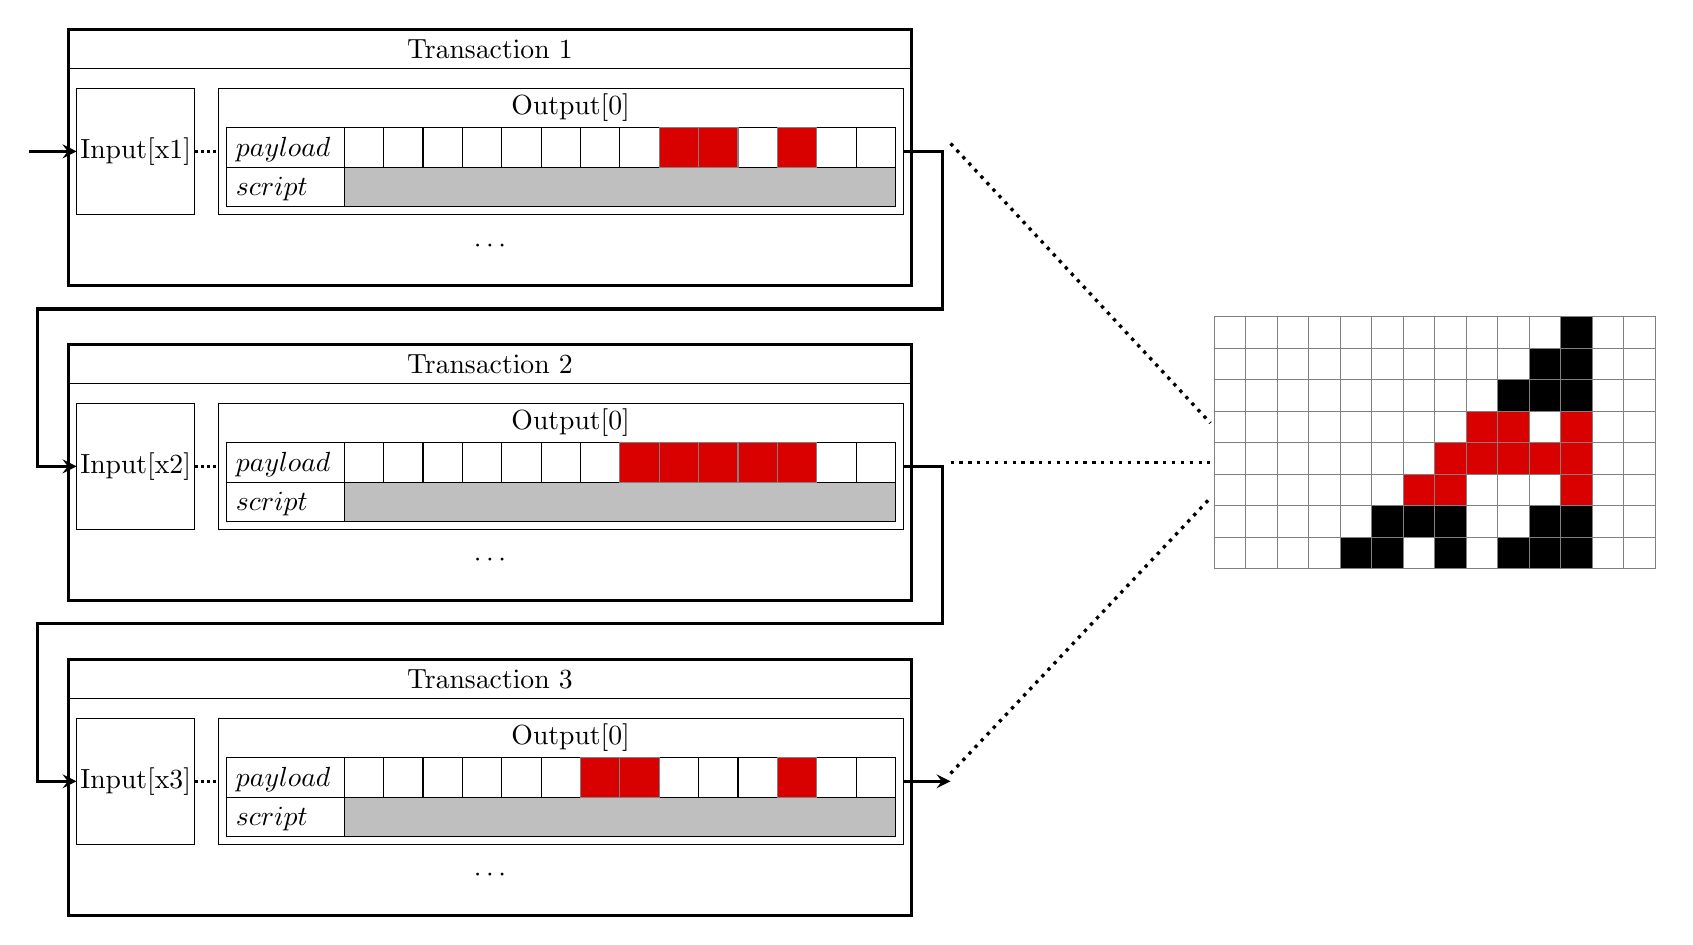
\begin{tikzpicture}[
        X/.style={draw=gray, minimum size=4mm, outer sep=0pt},
        B/.style={X, fill},
        C/.style={X, fill=black!15!red},
        D/.style={X, fill=black!15!red},
        E/.style={X, fill=black!15!red},
        mymatrix/.style={matrix of nodes, row
            sep=-\pgflinewidth,
            column sep=-\pgflinewidth, nodes={X}, nodes in
        empty cells}
    ]

    \def\h{0.5}
    \txbox{0,0}{1}
    \txbox{0,-4}{2}
    \txbox{0,-8}{3}
    \chainArr{8.6}{-0.3}{-1.9}{-4.3}
    \chainArr{8.6}{-4.3}{-1.9}{-8.3}
    \draw[very thick, dotted](9.2,-0.2) -- (12.5,-3.75);
    \draw[very thick, dotted](9.2,-4.25) -- (12.5,-4.25);
    \draw[very thick, dotted](9.2,-8.2) -- (12.5,-4.7);
    \draw[very thick, ->, >=stealth](8.6,-8.3) -- (9.2,-8.3);
    \draw[very thick, ->, >=stealth](-2.5,-0.3) -- (-1.9,-0.3);

    \foreach \i in {5.5,6,7}
    {
        \draw[C] ($(\i,0)$) rectangle ($({\i+\h},-\h)$);
    }

    \foreach \i in {5,5.5,6,6.5,7}
    {
        \draw[D] ($(\i,-4)$) rectangle ($({\i+\h},-4-\h)$);
    }
    \foreach \i in {4.5,5, 7}
    {
        \draw[E] ($(\i,-8)$) rectangle ($({\i+\h},-8-\h)$);
    }
    \matrix at (15.35,-4) [mymatrix]{
        &&&&&&&&&&&|[B]|&&\\
        &&&&&&&&&&|[B]|&|[B]|&&\\
        &&&&&&&&&|[B]|&|[B]|&|[B]|&&\\
        &&&&&&&&|[C]|&|[C]|&&|[C]|&&\\
        &&&&&&&|[D]|&|[D]|&|[D]|&|[D]|&|[D]|&&\\
        &&&&&&|[E]|&|[E]|&&&&|[E]|&&\\
        &&&&&|[B]|&|[B]|&|[B]|&&&|[B]|&|[B]|&&\\
        &&&&|[B]|&|[B]|&&|[B]|&&|[B]|&|[B]|&|[B]|&&\\
    };
    \end{tikzpicture}
\end{document}
